%%%%%%%%%%%%%%%%%%%%%%%%%%%%%%%%%%%%%%%%%
% Jacobs Landscape Poster
% LaTeX Template
% Version 1.1 (14/06/14)
%
% Created by:
% Computational Physics and Biophysics Group, Jacobs University
% https://teamwork.jacobs-university.de:8443/confluence/display/CoPandBiG/LaTeX+Poster
% 
% Further modified by:
% Nathaniel Johnston (nathaniel@njohnston.ca)
%
% This template has been downloaded from:
% http://www.LaTeXTemplates.com
%
% License:
% CC BY-NC-SA 3.0 (http://creativecommons.org/licenses/by-nc-sa/3.0/)
%
%%%%%%%%%%%%%%%%%%%%%%%%%%%%%%%%%%%%%%%%%

%----------------------------------------------------------------------------------------
%	PACKAGES AND OTHER DOCUMENT CONFIGURATIONS
%----------------------------------------------------------------------------------------

\documentclass[final]{beamer}

\usepackage[scale=1.12]{beamerposter} % Use the beamerposter package for laying out the poster

\usetheme{confposter} % Use the confposter theme supplied with this template

\setbeamercolor{block title}{fg=ngreen,bg=white} % Colors of the block titles
\setbeamercolor{block body}{fg=black,bg=white} % Colors of the body of blocks
\setbeamercolor{block alerted title}{fg=white,bg=dblue!70} % Colors of the highlighted block titles
\setbeamercolor{block alerted body}{fg=black,bg=dblue!10} % Colors of the body of highlighted blocks
% Many more colors are available for use in beamerthemeconfposter.sty

%-----------------------------------------------------------
% Define the column widths and overall poster size
% To set effective sepwid, onecolwid and twocolwid values, first choose how many columns you want and how much separation you want between columns
% In this template, the separation width chosen is 0.024 of the paper width and a 4-column layout
% onecolwid should therefore be (1-(# of columns+1)*sepwid)/# of columns e.g. (1-(4+1)*0.024)/4 = 0.22
% Set twocolwid to be (2*onecolwid)+sepwid = 0.464
% Set threecolwid to be (3*onecolwid)+2*sepwid = 0.708

\newlength{\sepwid}
\newlength{\onecolwid}
\newlength{\twocolwid}
\newlength{\threecolwid}
\setlength{\paperwidth}{48in} % A0 width: 46.8in
\setlength{\paperheight}{36in} % A0 height: 33.1in
\setlength{\sepwid}{0.024\paperwidth} % Separation width (white space) between columns
\setlength{\onecolwid}{0.22\paperwidth} % Width of one column
\setlength{\twocolwid}{0.464\paperwidth} % Width of two columns
\setlength{\threecolwid}{0.708\paperwidth} % Width of three columns
\setlength{\topmargin}{-0.8in} % Reduce the top margin size
%-----------------------------------------------------------

\usepackage{graphicx}  % Required for including images

\usepackage{booktabs} % Top and bottom rules for tables

%----------------------------------------------------------------------------------------
%	TITLE SECTION 
%----------------------------------------------------------------------------------------


\title{Simulating Timing Resolution Effects of Scintillation Geometry for the M9 Prototype
Muon Spectrometer} % Poster title

\author{Jerin Roberts, Dr. Mark Paetkau and Dr. Syd Krietzman} % Author(s)

\institute{Physical Sciences  Thompson Rivers University} % Institution(s)

%----------------------------------------------------------------------------------------

\begin{document}

\addtobeamertemplate{block end}{}{\vspace*{1ex}} % White space under blocks
\addtobeamertemplate{block alerted end}{}{\vspace*{1ex}} % White space under highlighted (alert) blocks

\setlength{\belowcaptionskip}{1ex} % White space under figures
\setlength\belowdisplayshortskip{1ex} % White space under equations

\begin{frame}[t] % The whole poster is enclosed in one beamer frame

\begin{columns}[t] % The whole poster consists of three major columns, the second of which is split into two columns twice - the [t] option aligns each column's content to the top

\begin{column}{\sepwid}\end{column} % Empty spacer column

\begin{column}{\onecolwid} % The first column

%----------------------------------------------------------------------------------------
%	OBJECTIVES
%----------------------------------------------------------------------------------------



\begin{alertblock}{Objective}

\begin{itemize}
\item Simulate attainable resolution of a prototype spectrometer.
\end{itemize}

\end{alertblock}

%----------------------------------------------------------------------------------------
%	INTRODUCTION
%----------------------------------------------------------------------------------------
\begin{block}{Introduction}

Muon Spectrometers are designed to probe the fine magnetic structures of materials being studied. At the Canadian National Subatomic Physics Laboratory TRIUMF, muons are generated using the institutions large cyclotron. 

\begin{figure}
{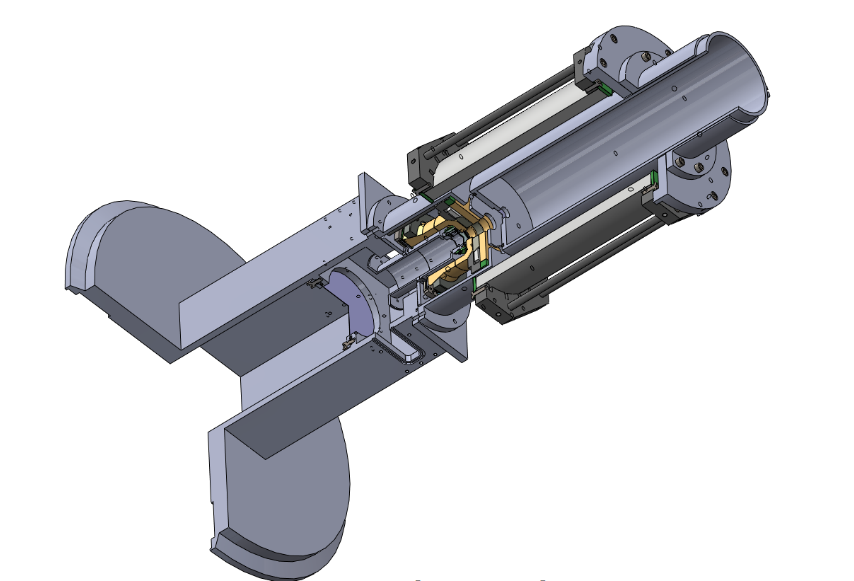
\includegraphics[height=15cm]{spect}}
\caption{CAD model of M9 Muon Spectrometer}
\end{figure}
The muons are embedded into materials at low energies (5-50MeV) \cite{musr}. While embedded in the sample the muon spin precesses about the local internal magnetic field \cite{mu}. The Muons then decay releasing positrons which pass through the scintillator generating a burst of light. 
\begin{figure}
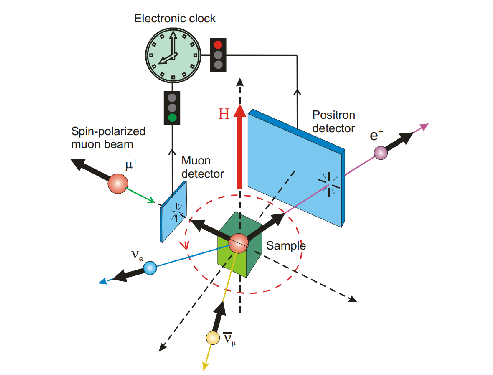
\includegraphics[width=\linewidth]{spec}
\caption{Displays Simplified Diagram of a transverse field muon spectrometer \cite{mu} }
\end{figure}


 The time difference between light detection points allows for the positron trajectory to be reconstructed which gives information about the shape of the internal magnetic structure of the sample.

\end{block}

%------------------------------------------------



%----------------------------------------------------------------------------------------

\end{column} % End of the first column

\begin{column}{\sepwid}\end{column} % Empty spacer column

\begin{column}{\twocolwid} % Begin a column which is two columns wide (column 2)

\begin{columns}[t,totalwidth=\twocolwid] % Split up the two columns wide column

\begin{column}{\onecolwid}\vspace{-.6in} % The first column within column 2 (column 2.1)

%----------------------------------------------------------------------------------------
%	MATERIALS
%----------------------------------------------------------------------------------------


\begin{block}{Simulation}

A simulation was written in C++ and analyzed using ROOT. The architecture enables simulation of scintillation pieces generated using 3D CAD programs. The simulation generates random photons along a positron trajectory through the scintillator which propagate until they reach a Silicon Photomultiplier (SiPM).


\begin{figure}
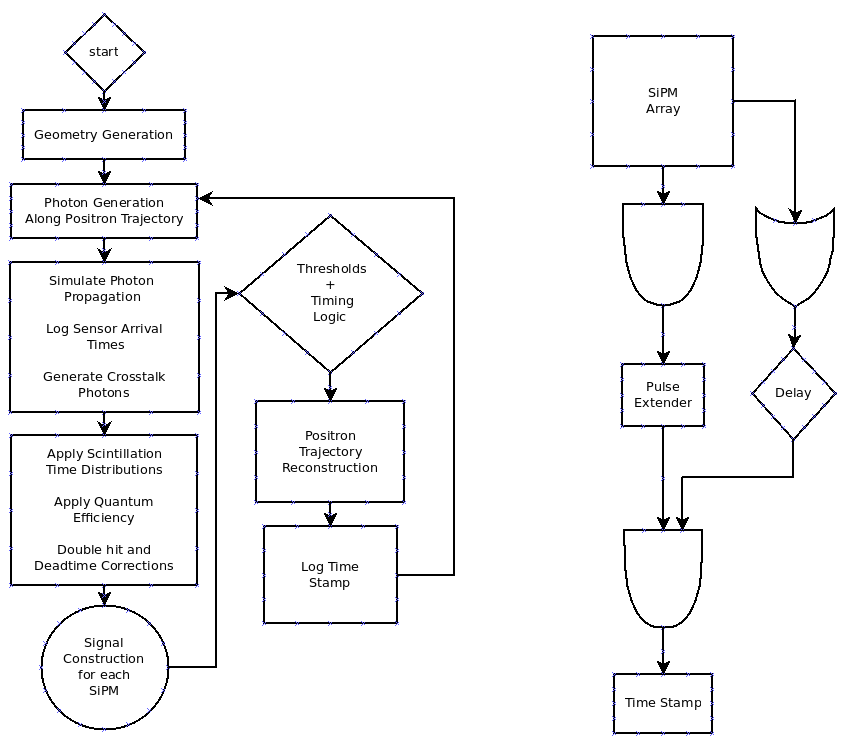
\includegraphics[height=21cm]{dia}
\caption{Simulation flow chart with logic discrimination}
\end{figure}
 Each photon is time stamped and checked for double hits. Cross talk and scintillation probabilities are used to adjust each stamp which is then used to generate a pulse. The sum of the pulses from each photon hit forms the final signal. A threshold is applied which gives a time of the incoming pulse. The time of this pulse is stored and the simulation reiterates a new positron event.
 
\begin{figure}
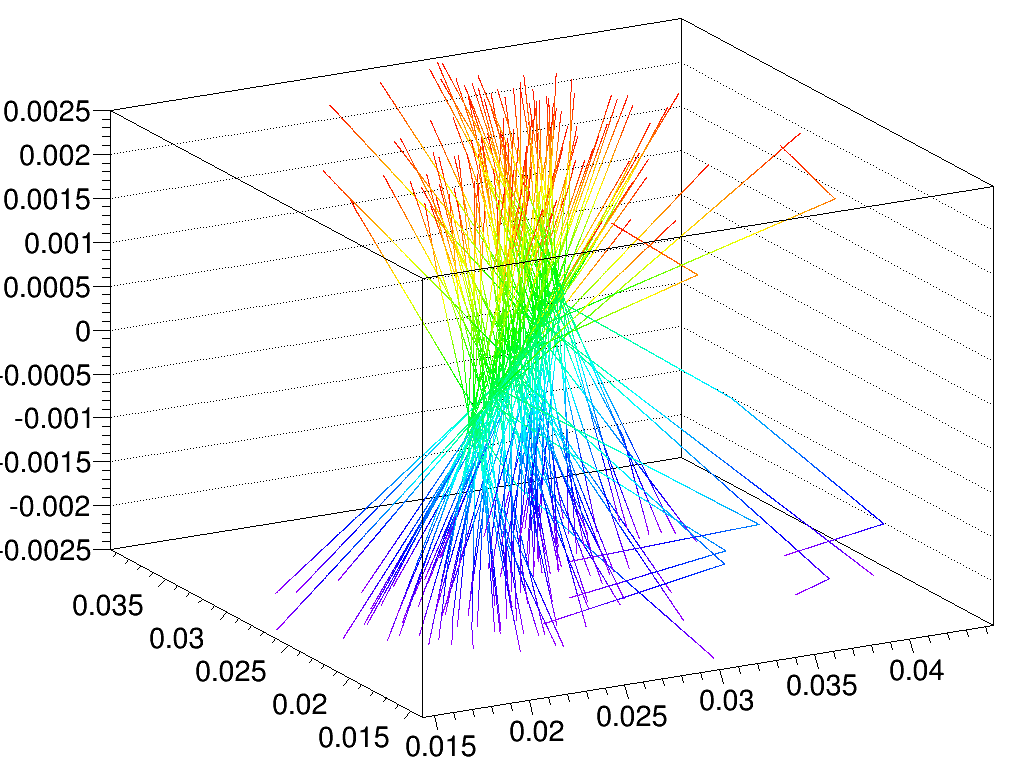
\includegraphics[height=21cm]{picsim}
\caption{Photons being randomly generated along a positron trajectory}
\end{figure} 
 
\end{block}


%----------------------------------------------------------------------------------------

\end{column} % End of column 2.1

\begin{column}{\onecolwid}\vspace{-.6in} % The second column within column 2 (column 2.2)

%----------------------------------------------------------------------------------------
%	METHODS
%----------------------------------------------------------------------------------------
\begin{block}{Results}


\space
\space
\space
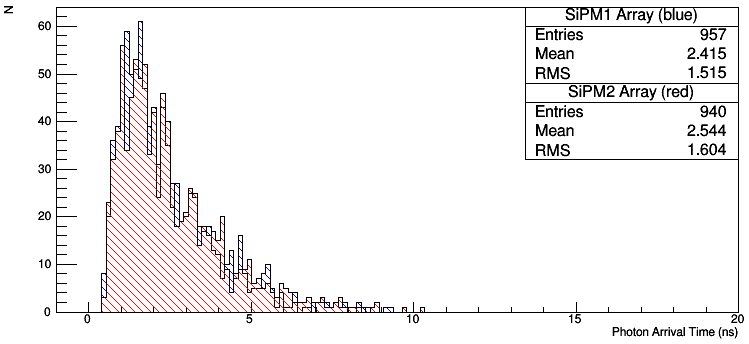
\includegraphics[height=12cm]{d3}
\newline
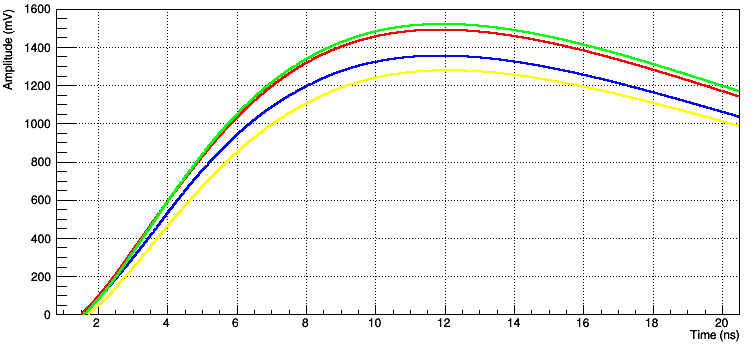
\includegraphics[height=12.15cm]{d2}

\begin{figure}
\caption{Output of a single positron event. a) Displays all photon arrival times with adjustments. b) SiPM output signals.}
\end{figure}

\centering
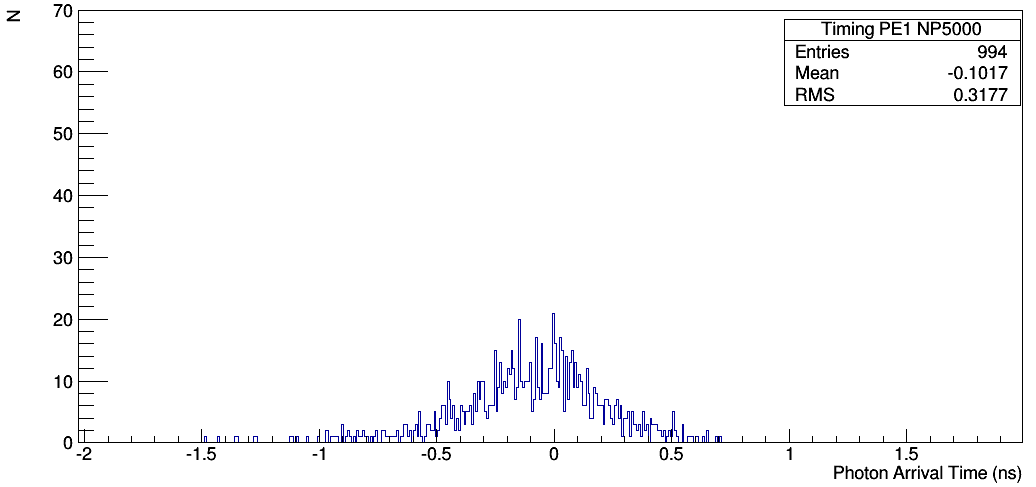
\includegraphics[height=11.2cm]{d6}
\newline
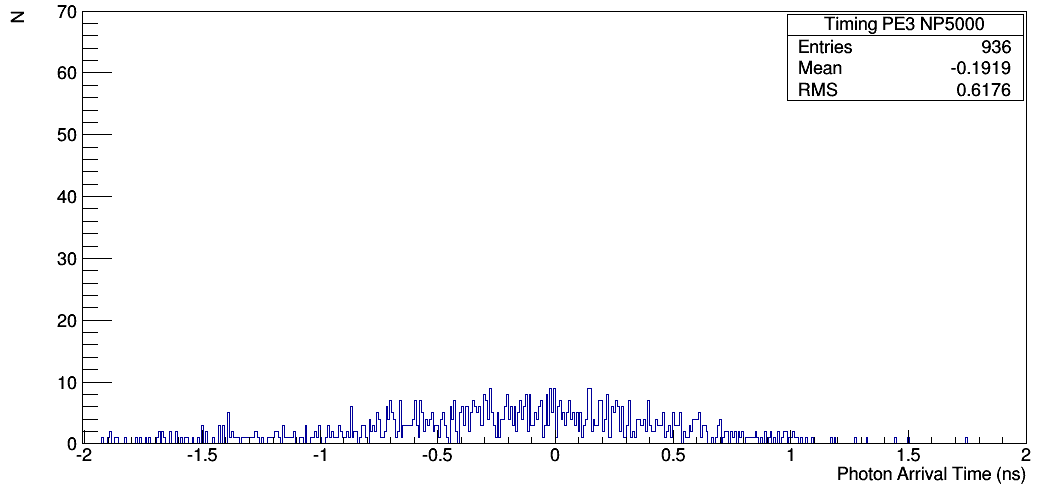
\includegraphics[height=11.2cm]{d7}
\newline
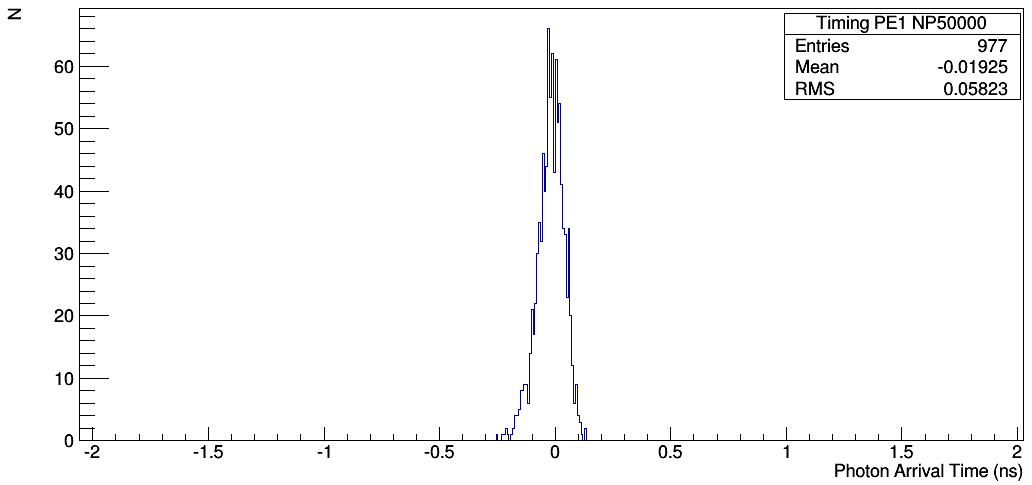
\includegraphics[height=11.2cm]{d4}
\newline

\begin{figure}


\caption{The timing results of multiple positron events for specific energies (5MeV to 50MeV) and thresholds (1PE to 3PE)}
\end{figure}





\end{block}

%----------------------------------------------------------------------------------------


%----------------------------------------------------------------------------------------

\end{column} % End of column 2.2

\end{columns} % End of the split of column 2 - any content after this will now take up 2 columns width

%----------------------------------------------------------------------------------------
%	IMPORTANT RESULT
%----------------------------------------------------------------------------------------



%----------------------------------------------------------------------------------------

\begin{columns}[t,totalwidth=\twocolwid] % Split up the two columns wide column again

\begin{column}{\onecolwid} % The first column within column 2 (column 2.1)

%----------------------------------------------------------------------------------------
%	MATHEMATICAL SECTION
%----------------------------------------------------------------------------------------



%----------------------------------------------------------------------------------------

\end{column} % End of column 2.1

\begin{column}{\onecolwid} % The second column within column 2 (column 2.2)

%----------------------------------------------------------------------------------------
%	RESULTS
%----------------------------------------------------------------------------------------

 
\end{column} % End of column 2.2

\end{columns} % End of the split of column 2




\end{column} % End of the second column

\begin{column}{\sepwid}\end{column} % Empty spacer column

\begin{column}{\onecolwid} % The third column

%----------------------------------------------------------------------------------------
%	CONCLUSION
%----------------------------------------------------------------------------------------

\begin{block}{Conclusion}
The results of the simulation conclude that a 60 picosecond resolution can be attained for the Sensl B-series SiPM given the energy of the positron is sufficiently high and given optimal thresholds are used. It was shown cylindrical scintillation pieces had small contributions to timing as the geometry is isotropic, therefore timing largely dependent on the single photon response of SiPM and methods of discrimination. The Sensl C-series SiPM's (unavailable at the time) due to their low noise capabilities could provide lower positron energy window while still attaining a ~60ps resolution.


\end{block}
\begin{alertblock}{Important Result}

The simulation suggests a 60 ps resolution is attainable using the low noise Silicon photomultipliers with digital logic discrimination.

\end{alertblock}

%----------------------------------------------------------------------------------------
%	ADDITIONAL INFORMATION
%----------------------------------------------------------------------------------------


%----------------------------------------------------------------------------------------
%	REFERENCES
%----------------------------------------------------------------------------------------

\begin{block}{References}

\begin{thebibliography}{99} % Beamer does not support BibTeX so references must be inserted manually as below
\bibitem[1]{mu} Jeff E. Sonier  (2014)
\newblock  Muon Spin Rotation, Relaxation, Resonance 
\newblock http://musr.ca/intro/musr/muSRBrochure.pdf


\bibitem[2]{musr} muSR general homepage (2012)
\newblock http://musr.ca/


\bibitem[3]{mu2} Joelle Barral  (2008)
\newblock Study of Silicon Photomultipliers
\newblock http://www.stanford.edu/



\end{thebibliography}

\end{block}

%----------------------------------------------------------------------------------------
%	ACKNOWLEDGEMENTS
%----------------------------------------------------------------------------------------

\setbeamercolor{block title}{fg=red,bg=white} % Change the block title color

\begin{block}{Acknowledgements}

\small{\rmfamily{Special Thanks goes to Syd Krietzman and Mark Paetkau for providing resources, information and for overlooking this project}} \\

\end{block}

%----------------------------------------------------------------------------------------
%	CONTACT INFORMATION
%----------------------------------------------------------------------------------------

\setbeamercolor{block alerted title}{fg=black,bg=norange} % Change the alert block title colors
\setbeamercolor{block alerted body}{fg=black,bg=white} % Change the alert block body colors

\begin{alertblock}{Contact Information}

\begin{itemize}
\item Jerin Roberts
\item Email: \href{mailto:john@smith.com}{robertsj@snolab.ca}
\item Phone: 250-682-6536


\end{itemize}



\end{alertblock}

\begin{center}
\begin{tabular}{ccc}

\includegraphics[width=0.5\linewidth]{tri} & \hfill & 
\includegraphics[width=0.2\linewidth]{tru}

\end{tabular}
\end{center}
\begin{center}
\begin{tabular}{ccc}

\includegraphics[width=0.4\linewidth]{root}& \hfill & 
\includegraphics[width=0.4\linewidth]{cmms}

\end{tabular}
\end{center}

%----------------------------------------------------------------------------------------

\end{column} % End of the third column

\end{columns} % End of all the columns in the poster

\end{frame} % End of the enclosing frame

\end{document}
